% % % % % % % % % % % % % % % % % % % % % % % % % % % % % % % % % % % % % % % % 
% Formelsammlung von LaTeX4EI									
%
% @encode: 	UTF-8, tabwidth = 4, newline = LF
% @author:	Lukas Kompatscher
% @date:		
%
% % % % % % % % % % % % % % % % % % % % % % % % % % % % % % % % % % % % % % % % 

%-------------------------------------------%
%  Stochastische Signale MATLAB Praktikum	%
%~~~~~~~~~~~~~~~~~~~~~~~~~~~~~~~~~~~~~~~~~~~%

% Document Class ===============================================================
\documentclass[deutsch]{latex4ei/latex4ei_sheet}

% set document information
\title{Stochastische \\ Signale Praktikum}
\author{Lukas Kompatscher}			
\myemail{lukas.kompatscher@tum.de}		

\usepackage{listings}
\usepackage{color} %red, green, blue, yellow, cyan, magenta, black, white
\definecolor{mygreen}{RGB}{28,172,0} % color values Red, Green, Blue
\definecolor{mylilas}{RGB}{170,55,241}

\lstset{language=Matlab,%
	%basicstyle=\color{red},
	breaklines=true,%
	morekeywords={matlab2tikz},
	keywordstyle=\color{blue},%
	morekeywords=[2]{1}, keywordstyle=[2]{\color{black}},
	identifierstyle=\color{black},%
	stringstyle=\color{mylilas},
	commentstyle=\color{mygreen},%
	showstringspaces=false,%without this there will be a symbol in the places where there is a space
%	numbers=left,
	numberstyle={\tiny \color{black}},% size of the numbers
	numbersep=9pt, % this defines how far the numbers are from the text
	emph=[1]{for,end,break},emphstyle=[1]\color{red}, %some words to emphasise
	%emph=[2]{word1,word2}, emphstyle=[2]{style},    
}


% DOCUMENT_BEGIN ===============================================================
\begin{document}

\maketitle

% SECTION ======================================================================
\section{Allgemeine Befehle}
% ==============================================================================

\begin{sectionbox}
	\subsection{Standardbefehle}
	\begin{tablebox}{ll}
		Befehl & Funktion\\ \cmrule
		save(\textit{filename, variable}) & speichert \textit{variable} in matfile\\
		load(\textit{filename}) & lädt Variable aus matfiel \\
		clear \textit{variable} & löscht \textit{variable}\\
		clear all & löscht alle Variablen im Workspace\\
		clc & löscht Inhalt des Kommandofensters\\
		doc \textit{expression} & Hilfedatei zu \textit{expression}\\
		help \textit{expression} & Kurzhilfe zu \textit{expression} \\

	\end{tablebox}
\end{sectionbox}

%\begin{sectionbox}
%	\subsection{Datentypkonvertierung (Karsten)}
%	\begin{tablebox}{ll}
%		
%		Befehl & Funktion \\\cmrule
%		double(\textit{array}) & Umwandlung von \textit{array} in double\\
%		
%	\end{tablebox}
%\end{sectionbox}

\begin{sectionbox}
	\subsection{Allgemeine Rechenoperationen}
	\begin{tablebox}{ll}
		
		Befehl & Funktion \\\cmrule
		mod(x,y) & x modulo y (immer positiv)\\
		rem(x,y) & x modulo y (vorzeichenabhängig)\\
		sqrt(x) & $ \sqrt{x}$\\
		exp(x) & $e^x$\\
		log(x) & Natürlicher Logarithmus $\ln(x)$\\
		floor(x) & Abrunden auf Integer\\
		ceil(x) & Aufrunden auf Integer\\
		sum(x) & Summe über Werte des Vektors x\\
		prod(x) & Produkt über Werte des Vektors x\\
		min(x) & kleinster Wert des Vektors x\\
		max(x) & größter Wert des Vektors x\\
		all(x) & 1 für keine 0 in Vektor x\\
		any(x) & 1 für eine Nicht-0 in Vektor x\\
		mean(x) & Mittelwert des Vektors x\\
		sign(x) & Vorzeichen von x (0 wenn x=0)\\
		abs(x) & Betrag von x\\
	\end{tablebox}
\end{sectionbox}

\begin{sectionbox}
	\subsection{Operatoren}
	\begin{tablebox}{ll}
		Operator & Funktion \\\cmrule
		a\textgreater b & Gibt logisch 1 zurück wenn $a>b$, sonst 0\\
		a\textgreater=b & Gibt logisch 1 zurück wenn $a\ge b$, sonst 0\\
		a==b & Gibt logisch 1 zurück wenn $a=b$, sonst 0\\
		a\textasciitilde =b & Gibt logisch 1 zurück wenn $a\ne b$, sonst 0\\
		a*b & Matrix-Matrix-Multiplikation von a und b\\
		a.*b & Elementenweise Multiplikation von a und b\\
		a(a\textgreater=0) & Gibt Teilvektor von a zurück, wo der Wert $\ge 0$
	\end{tablebox}
\end{sectionbox}

\begin{sectionbox}
	\subsection{Komplexe Zahlen}
	\begin{tablebox}{ll}
		
		Befehl & Funktion \\\cmrule
		complex(a,b) & $a+jb$ \\
		real(z) & Realteil von z\\
		imag(z) & Imaginärteil von z\\
		abs(z) & Betrag/Komplexe Amplitude von z\\
		angle(z) & Phase von z\\
		conj(z) & konjugiert komplex von z\\
		
	\end{tablebox}
\end{sectionbox}

\begin{sectionbox}
	\subsection{Trigonometrische Funktionen}
	\begin{tablebox}{ll}
		Befehl & Funktion \\\cmrule
		sin(x) , cos(x), tan(x) & x in Bogenmaß\\
		sind(x), cosd(x), tand(x) & x in Grad\\
		asin(x), acos(x), atan(x) & Arcusfunktionen (Rad)\\
		asind(x), acosd(x), antans(x) & Arcusfunktionen (Grad)\\
		
	\end{tablebox}
\end{sectionbox}

% SECTION ======================================================================
\section{Matrizenrechnung}
% =============================================================================
\begin{sectionbox}
	\subsection{Rechenoperationen}
	\begin{tablebox}{ll}
		Befehl & Funktion \\\cmrule
		{[}a b c{]} & Zeilenvektor (bzw. vertikales aneinanderreihen)\\
		{[}a; b; c{]} & Spaltenvektor (bzw. horizontales aneinanderreihen)\\
		{[}a b c; d e f; g h i{]} & 3x3-Matrix\\
		{[}a b{]} = size(\ma A) & Dimensionen der Matrix (a Zeilen, b Spalten)\\
		inv($\ma A$) & inverse Matrix von $\ma A$\\
		$\ma A$' & $\ma A^\top$ (transponiert konjugiert komplex)\\
		$\ma A$.' & $\ma A^\top$ (transponiert)\\
		$\ma A\setminus \vec b $ & löst $\ma A \vec x= \vec b$\\
		$\ma A$(m,n) & Element $\ma A_{m,n}$\\
		$\ma A$(m,:) & m-te Zeile\\
		$\ma A$(:,n) & n-te Spalte\\
		$\ma A$(Bedingung) & Alle Element in A, auf die die Bedingung zutrifft\\
		find(\ma A) & lokalisiert Nicht-Null-Elemente (Indizes)\\
		det(\ma A) & Determinante von A \\
		rank(\ma A) & Rang (Anzahl unabhängiger von A \\
		\lbrack V,D\rbrack = eig(\ma A) & Eigenwerte (D) und Eigenvektoren (V) von A \\
		(a:b:c) & Vektor von a bis c mit Schrittweite b\\
		linspace(a,b,n) & n Werte im gleichen Abstand von a bis b\\
		norm(x) & eukl. Norm des Vektors x\\
		sum($\ma A$) & Summer der Werte über Spaltenwerte\\
		sum($\ma A$,2) & Summer der Werte über Zeilenwerte\\
		mean($\ma A$) & Mittelwert der Spaltenwerte\\
		mean($\ma A$,2) & Mittelwert der Zeilenwerte\\
		numel($\ma A$) & Anzahl der Elemente in $\ma A$\\
	\end{tablebox}
	
	Komponentenweises Rechnen durch einen Punkt vor einem Operator\\
	Bsp: $\ma A$.\^{}2 quadriert jedes Element der Matrix $\ma A$\\
	Inlinefunktion: @(x)(f(x))
\end{sectionbox}

\begin{sectionbox}
	\subsection{Spezielle Matrizen}
	\begin{tablebox}{ll}
		Befehl & Funktion \\\cmrule
		eye(m,n) & $m\times n$ Einheitsmatrix\\
		zeros(m,n) & $m\times n$ 0-Matrix\\
		ones(m,n) & $m\times n$ 1-Matrix\\
		diag($\vec x$) & Diagonalmatrix mit den Werten von $\vec x$\\
		rand(m,n) & $m\times n$ Zufallsmatrix (Werte: 0-1)\\
		randi(imax,m,n) & integer Zufallsmatrix mit max. imax\\
		magic(n) & $n\times n$ magisches Quadrat
	\end{tablebox}
\end{sectionbox}

% SECTION ======================================================================
\section{Schleiflab}
% =============================================================================
\vspace{-0.0em}
\begin{sectionbox}
	\begin{tablebox}{p{0.5\textwidth}p{0.5\textwidth}}
		while: & for: \\ \cmrule
		\emph{while} expression & \emph{for} i=0:1:20\\
		statements & statements \\
		\emph{end} & \emph{end}\\
	\end{tablebox}
	Schleife vorzeitig verlassen mit break
\end{sectionbox}

% SECTION ======================================================================
\section{Plotten}
% =============================================================================
\begin{sectionbox}
	\begin{tablebox}{ll}
		Befehl & Funktion \\\cmrule
		plot(x,y,'prop') & Plottet x und y mit Farbe/Symbol 'prop'\\
		stem(y) & Plottet diskrete y Werte (nicht verbunden)\\
		bar(x,y) & Plottet x und y in einem Balkendiagramm\\
		xlim([a b]) & Begrenzt Bereich der x-Achse auf [a,b]\\
		ylim([c d]) & Begrenzt Bereich der y-Achse auf [c,d]\\
		axis([a b c d]) & Kombination aus xlim + ylim \\
		xlabel('Name') & Benennt x-Achse\\
		ylabel('Name') & Benennt y-Achse\\
		titel('Titel') & Tituliert den Plot\\
		subplot(H,B,Position) & Selektiert Plot in Figure mit H x B Plots\\
	\end{tablebox}
	\emph{Beispiel:}
	\begin{lstlisting}[gobble=4]
	figure(1);				% new figure
	clf;					% clear old figures
	plot(x, y, 'k');		% plot y(x) in black 'k'
	hold on;				% more plots in same figure
	plot(x, z, 'ro')		% plot z(x) in red circles
	legend('y', 'z')		% names of plots
	hold off;
	\end{lstlisting}
\end{sectionbox}

% SECTION ======================================================================
\section{Stochastische Zufallsvariablen}
% ==============================================================================

\begin{sectionbox}
	\subsection{Realisierung von Standardmodellen}
	\begin{tablebox}{ll}
		Befehl & $m\times n$-Realisierung einer \dots \\\cmrule
		rand(m,n) & gleichverteile ZV (Werte: 0-1)\\
		randn(m,n) & Standardnormalverteilung $\mathcal N(0, 1)$\\
		gamrnd(k,t,m,n) & gammaverteile ZV, shape k, scale t\\
		binornd(n,p,m,n) &  Binomialverteilung mit Parameter n, p\\
		binornd(1,p,m,n) &  Bernoulliverteilung mit Wahrscheinlichkeit p\\
		geornd(p,m,n) & Geometrische Verteilung mit Wahrsch. p\\
		exprnd(1/lambda,m,n) & Exponentialverteilung mit Parameter $\lambda$\\
	\end{tablebox}
	\emph{Beispiele:}
	\begin{tablebox}{ll}
		Befehl & Ergebnis \\\cmrule
		2*rand+1 & gleichverteile ZV im Bereich [1,3]\\
		plot(y,unifpdf((y-1)/2)/2) & plottet PDF der oberen ZV\\
		plot(x,unifpdf(2*x)*2) & PDF einer gv. ZV im Bereich [0,0.5]\\
		sigma*randn+mu & Realisierung der Normalv. $\mathcal N(\mu, \sigma^2)$
	\end{tablebox}
\end{sectionbox}

\begin{sectionbox}
	\subsection{Wahrscheinlichkeitsdichtefunktion (PDF) $f_{\X}(x)$}
	
	\begin{tablebox}{ll}
		Befehl & PDF an den Stellen x einer \dots \\\cmrule
		unifpdf(x,a,b) & Gleichverteilung im Intervall [a,b]\\
		poisspdf(x,lambda) & Poissonverteilung mit Parameter $\lambda$\\
		normpdf(x,mu,sigma) & Normalverteilung mit Parameter mu und sigma\\
		gampdf(x,k,t) & Gammaverteilung mit shape k und scale t\\
		
	\end{tablebox}
\end{sectionbox}

\begin{sectionbox}
	\subsection{Kommulative Verteilungsfunktion (CDF) $F_{\X}(x)$}
	\begin{tablebox}{ll}
		Befehl & CDF an den Stellen x einer \dots \\\cmrule
		unifcdf(x,a,b) & Gleichverteilung im Intervall [a,b]\\
		poisscdf(X,lambda) & Poissonverteilung mit Parameter $\lambda$\\
		normcdf(X,mu,sigma) & Normalverteilung mit Parameter $\mu$ und $\sigma$\\
		cdfplot(X) & Schätzt und plottet CDF von X\\
	\end{tablebox}
\end{sectionbox}


% SECTION ======================================================================
\section{Analyse von Zufallsvariablen}
% ==============================================================================
\begin{sectionbox}
	\subsection{Schätzung von Paramtern einer Zufallsvariable X}
	x ist ein Vektor von Realisierungen von X
	\begin{tablebox}{ll}
		Befehl & Funktion\\ \cmrule
		mean(x) & Schätzt Erwartungswert $\mu$ der ZV X\\
		var(x) & Schätzt Varianz $\Var(X)$ der ZV X\\
		std(x) & Schätzt die Standardabweichung $\sigma$ der ZV X\\
		length(x) & Anzahl der Realisierungen der ZV X\\
		mean(x.\^{}3) & Schätzung des 3. Moments der ZV X
	\end{tablebox}
\end{sectionbox}

\begin{sectionbox}
	\subsection{Histogramm}
	\begin{tablebox}{lp{0.7\textwidth}}
		Befehl & Funktion \\ \cmrule
		hist(A) & Teilt A in 10 gleiche Bereiche (Bins) und zählt die Elemente im jeweiligen Bin\\
		hist(A,b) & Teilt A in b gleiche Bereiche (Bins) und zählt die Elemente im jeweiligen Bin\\
		hist(A,centers) & Zählt die Elemente in den Bins um den Einträgen in centers\\
		\lbrack n,centers\rbrack =hist(...) & Gibt in Anzahl der Elemente in n zurück und die Position der Bins in centers\\
		bar(hist(...)) & Erstellt ein Balkendiagramm des Histogramms
	\end{tablebox}
\end{sectionbox}

% SECTION ======================================================================
\section{Signalverarbeitung}
% ==============================================================================
\begin{sectionbox}
	\subsection{Audiosignalverarbeitung}
	
	\begin{tablebox}{lp{0.65\textwidth}}
		Befehl & Funktion\\ \cmrule
		[a,b]=audioread('....') & Liest Audiodatei in Vektor a ein (Abtastrate b)\\
		sound(x,b) & Spielt das Signal in Vektor x (Abtastrate b) ab\\
		buffer(x,n) & Teilt Signalvektor x in nichtüberlappende Frames der Länge n\\
		buffer(x,n,p) & Teilt Signalvektor x in Frames der Länge n die sich um p überlappen
	\end{tablebox}
	\emph{Beispiel:}
	\begin{lstlisting}[gobble=4]
	buffer(1:12,5,3)
	%liefert ...
	ans =
	     0     0     2     4     6     8
	     0     1     3     5     7     9
	     0     2     4     6     8    10
	     1     3     5     7     9    11
	     2     4     6     8    10    12
	\end{lstlisting}
	
	\subsubsection{Lineare Systeme}
	\begin{tablebox}{lp{0.65\textwidth}}
		Befehl & Funktion\\ \cmrule
		conv(x,y) & Faltung zwischen Vektor x und y \\
	\end{tablebox}
%	\begin{lstlisting}[gobble=4]
%%	
%	\end{lstlisting}
	conv(x,y) gibt einen Vektor der Länge length(x) + length(y) - 1 zurück
\end{sectionbox}



% SECTION ======================================================================

\section{Begriffe}
\begin{sectionbox}
	\textbf{i.i.d.}\\
	Independent and identically distributed (unabhängig und gleichverteilt)\\\\
	\textbf{Ergodisch}\\
	Eine Zufallsfolge heißt ergodisch, wenn Mittelwerte über die Zeit (für
	eine einzelne gegebene Realisierung der Folge) zum gleichen Ergebnis führen wie
	Erwartungswertbildung (für einen einzelnen Zeitpunkt).\\\\
	\textbf{Klingonisch}\\
	Die klingonische Sprache ist die von Klingonen gesprochen Sprache. Sie ist im gesamten Klingonischen Imperium verbreitet.
	
\end{sectionbox}


% SECTION ======================================================================
\section{Kapitel 1}
% ==============================================================================
\begin{sectionbox}
	\subsection{Histogramm einer gleichverteilten ZV plotten}
	\lstinputlisting{matlab/hist_rand.m}
\end{sectionbox}

% SECTION ======================================================================
\section{Kapitel 2: Quantisierung und Transformation von ZV}
% ==============================================================================
\begin{sectionbox}
	\subsection{Beispielaufgabe}
	Gegeben sei eine Zufallsvariable $\X$, die im Intervall $[0, 1]$ gleichverteilt ist und eine Zufallsvariable $\Y=g(X)$, deren WDF mit der folgenden Funktion ausgewertet werden kann:
	\begin{lstlisting}[gobble=4]
	function f = mypdf(y)
	f=unifpdf(exp(y)).*exp(y);	
	\end{lstlisting}
	\emph{Folgerungen:}\\
	Die Funktion $g=g(x)=ln(x)$\\
	1000 Realisierungen von $\Y$ erzeugen: y=log(rand(1000,1));\\
\end{sectionbox}

\vfill

% SECTION ======================================================================
\section{Kapitel 3: Bedingte Verteilung}
% ==============================================================================
\begin{sectionbox}
	\subsection{Histogramm eines AWGN-Kanals}
	\parbox{3.3cm}{
	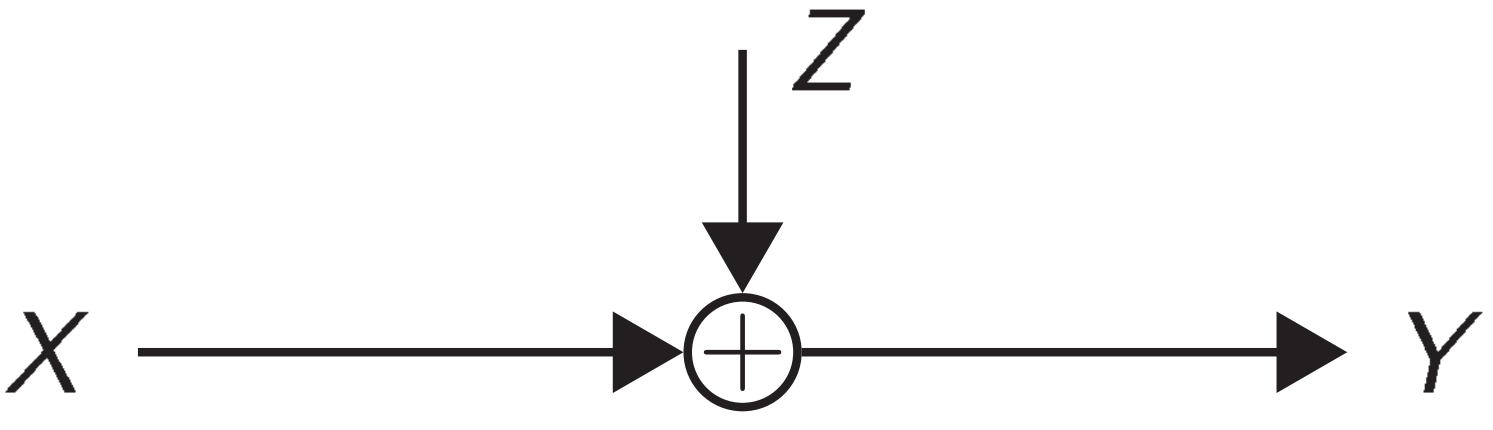
\includegraphics[width = 3cm]{img/awgn-channel.png}
	}
	\parbox{4cm}{
		$\X$ Eingangssignal\\
		$\Z = \mathcal N(0, \sigma^2)$ weißes Rauschen\\
		$\Y$ Ausgangssignal
		}
	\lstinputlisting{matlab/hist_out.m}
\end{sectionbox}

\begin{sectionbox}
	\subsection{Maximum-Likelihood-Detektion}
	\[ \max_{\hat x \in \{0,1\}}f_{\Y|\X}(y|\hat x) \]
	In unserem Fall: $\hat x = \begin{cases}
	0 & y\le \frac{1}{2}\\
	1 & y > \frac{1}{2}
	\end{cases}$
	Nachteil: Ignoriert das Wissen über die Eingangsverteilung.\\
	\begin{lstlisting}[gobble=4]
	function xhat = ml_detector(y)
	xhat=(y>0.5);
	\end{lstlisting}
	\textbf{Nachteil:} Ignoriert Wissen über die Eingangsverteilung \\
\end{sectionbox}

\begin{sectionbox}
	\subsection{Maximum-A-Posteriori-Detektion}
	\[\max_{\hat x \in \{0,1\}} p_{\X|\Y}(\hat x|y)\] mit
	\[p_{\X|\Y}(x|y)=\begin{cases}
	 \frac{p f_{\Z}(y-1)}{f_{\Y}(y)} & x=1\\
	\frac{(1-p)f_{\Z}(y)}{f_{\Y}(y)} & x=0\\
	0 & \text{sonst}
	\end{cases} 
	\Bigg\} = \frac{f_{\Y|\X}(y|x)p_{X}(x)}{f_{\Y}(y)}\]
	\begin{lstlisting}[gobble=4]
	function xhat = map_detector(y,p,sigma)
	xhat=(p*normpdf(y-1,0,sigma)>(1-p)*normpdf(y,0,sigma));
	\end{lstlisting}
	\textbf{Nachteil:} Die Verteilung der Zufallsvariable am Eingang muss bekannt sein\\
	\\

	\textbf{Spezialfall} der diskreten Gleichverteilung $p_{\X}(x)=\frac{1}{\abs{\Omega_{\X}}} \forall x \in \Omega_{\X}$:\\
	$p_{\X}$ für alle x gleich $\to$ kann aus der Entscheidungsregel gestrichen
	werden. ML äquivalent zu MAP
\end{sectionbox}

\section{Kapitel 4: Standardmodelle, Erwartungswert und Varianz}
\begin{sectionbox}
	\subsection{Modellierung für Mobilfunknetz}
	Überlagerung von Nutzern im Hotspot-Bereich (Normalverteilung) $\X_h, \Y_h$ und anderen Nutzern (Gleichverteilung) $\X_h, \Y_h$ mit der Bernoulli-verteilten ZV $B$.
	\[\X_m=\begin{cases}
	\X_h & \text{wenn } B=1\\
	\X_u & \text{wenn } B=0\\
	\end{cases} \qquad 
	\Y_m=\begin{cases}
	\Y_h & \text{wenn } B=1\\
	\Y_u & \text{wenn } B=0\\
	\end{cases}
	\]
	\lstinputlisting{matlab/mixed_positions.m}
\end{sectionbox}

\begin{sectionbox}
	\subsection{Empirische Realisierung von CDFs}	
	\parbox{3.5cm}{
		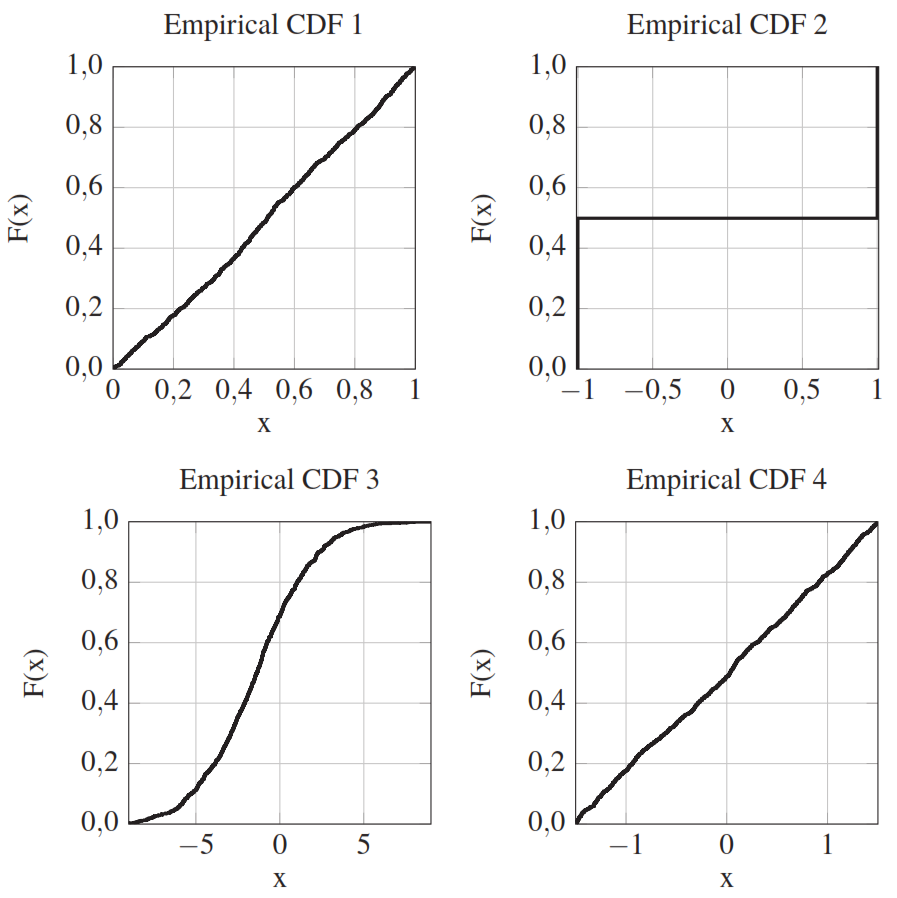
\includegraphics[width = 3.5cm]{img/cdf-sample.png}
	}
	\parbox{3.5cm}{
		(1)	cdfplot(rand(1000,1)); \\\\
		(2)	cdfplot(sign(rand(1000,1).5)); \\\\
		(3)	cdfplot(randn(1000,1)*3-1.5); \\\\
		(4)	cdfplot(rand(1000,1)*3-1.5);
		}
\end{sectionbox}

\section{Kapitel 5: Zufallsfolgen}
\begin{sectionbox}
	\subsection{Realisierung einer Zufallsfolge}
	$\X_{n+1}=\X_n+V_n \qquad \Y_{n+1}=\Y_n+W_n$ \\
	$V_n$ und $W_n$ sind i.i.d. Gleichverteilung mit Intervall $[-\delta;\delta]$\\
	Folgender Code aktualisiert die Positionen $(x_i,y_i)$ im Vektor pos
	\begin{lstlisting}[gobble=4]
	function pos=update_positions(pos,delta)
	pos=pos+2*delta*(rand(size(pos))-0.5);
	\end{lstlisting}
\end{sectionbox}

\section{Kapitel 6: Zufallsfolgen und lineare System}
\begin{sectionbox}
	\subsection{Signalgenerierung}
	\begin{lstlisting}[gobble=4]
	%Erstellt Sinussignal der Frequenz f1 mit der Amplitude A1,
	%ueberlagert mit weissen Rauschen mit Parameter sigma
	function x=create_signal(fS,T,f1,A1,sigma)
	t=1:T*fS;
	x=A1*sin(2*pi*f1/fS*t) + sigma*randn(1,fS*T);
	\end{lstlisting}
\end{sectionbox}

\begin{sectionbox}
	\subsection{Geschätzte Autokorrelationsfolge}
	Gegeben:
	\[\X_n=A_1 \sin(2\pi\frac{f}{f_s}n+\varphi_0)+\Z_n\]
	wobei $\varphi_0$ im Intervall $[0,2\pi]$ stetig gleichverteilt ist.\\
	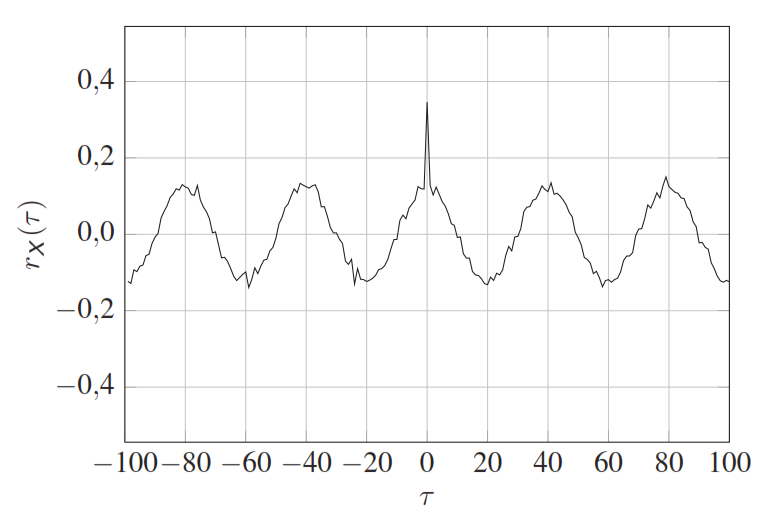
\includegraphics[width = \textwidth]{img/autokorrelation-graph.png}
	\begin{center}		
		Geschätzte Autokorrelationsfolge von $\X_n$\\
	\end{center}
	\textbf{Folgerung}
	\begin{itemize}
		\item Schätzung der Frequenz: $f=\frac{f_s}{40}$
		\item Der Peak bei $\tau = 0$ ist auf $\Z_n$ zurückzuführen
		\item $\E[Z_kZ_l]=0$ für $k\ne l$
	\end{itemize}
	


	
	
\end{sectionbox}

% DOCUMENT_END =================================================================
\end{document}


%TODO:
% - tic toc
